\chapter{Bewertung und Vergleich zu anderen Suchmaschinen}
 \label{sec:compareSearches}
Um einen Vergleich aufzustellen, werden Beispielanfragen mit der umgesetzten Suchmaschine durchgeführt und analysiert.
Anschliessend werden die Beispielanfragen auf externen Suchmaschinen durchgeführt.

\section{Bewertung der umgesetzten Suchmaschine}
Für jede Suche wird mindestens ein Teil der Resultat-Menge aufgelistet.

Da die umgesetzte Suche vers- oder genauer satzbasiert umgesetzt worden ist, müssen die Ergebnisse entsprechend manuell zu den vorgegebenen relevanten Bibelstellen gruppiert werden.
So kann schlussendlich ein sinnvoller Wert für die Precision und den Recall berechnet werden.
Ersichtlich wird dies in der Auswertung im \cref{subsec:index_abendmahl}.

% **********************************************************************************

\newpage
\subsection{Suche zum Thema Abendmahl}
\label{subsec:index_abendmahl}

\begin{table}[H]
	\centering
	\small\renewcommand{\arraystretch}{1.4}
	\rowcolors{1}{tablerowcolor}{tablebodycolor}
	%
	\captionabove{Suche: Vorkommen des Abendmahles}
	\label{tab:query_abendmahl}
	%
	\begin{tabularx}{0.9\textwidth}{ L{0.15\linewidth} | X  }%
		\hline
		Fragestellung: & \textit{Wo wurde das Abendmahl eingeführt?} \textit{Wo wird es erwähnt?}\\
		Anfrage-Typ: & \textit{Vers orientierte Anfrage}\\
		Beschreibung: & Der Nutzer will wissen, wo das Abendmahl erwähnt wird.\\
		Query: & \textit{brot AND leib}\\
		Erwartung: & 
		Vers und Stellenangabe:\footcite{Abendmahl_Jesu_Wikipedia_2016-05-30}
		\begin{itemize}[noitemsep]
			\item Mt 26, 26-28 \gls{lutLabel} ($\rightarrow$ gültiger Kontext: Vers 17–29)
			\item Mk 14, 22 \gls{lutLabel} ($\rightarrow$ gültiger Kontext: Vers 12-26)
			\item Lk 22, 17-20 \gls{lutLabel} ($\rightarrow$ gültiger Kontext: Vers 14–20)
			\item Joh 13,2–4 \gls{lutLabel}
			\item 1 Kor 11, 24 \gls{lutLabel} ($\rightarrow$ gültiger Kontext: Vers 23–27)
		\end{itemize}\\
		\hline
	\end{tabularx}
\end{table}

Die Suche nach dem Abendmahl (aus \cref{tab:query_abendmahl}), ergibt die folgenden 18 Ergebnisse.
Falsche Resultate werden durchgestrichen dargestellt. Mit gelb werden die explizit verlangten Bibelstellen hervorgehoben.
Bei den Resultaten die weder gelb noch durchgestrichen sind, stimmt der Context, aber sie waren nicht explizit verlangt.\\
\begin{itemize}[noitemsep]
	\item 1.	\st{Denn ein Brot ist's, so sind wir viele ein Leib, dieweil wir alle eines Brotes teilhaftig sind. - 1 Kor 10,17}
	\item 2.	Der gesegnete Kelch, welchen wir segnen, ist der nicht die Gemeinschaft des Blutes Christi? Das Brot, das wir brechen, ist das nicht die Gemeinschaft des Leibes Christi? - 1 Kor 10,16
	\item 3.	Welcher nun unwürdig von diesem Brot isset oder von dem Kelch des HERRN trinket, der ist schuldig an dem Leib und Blut des HERRN. - \hl{1 Kor 11,27}
	\item 4.	Und er nahm das Brot, dankte und brach's und gab's ihnen und sprach: Das ist mein Leib, der für euch gegeben wird; das tut zu meinem Gedächtnis. - \hl{Lk 22,19}
	\item 5.	Da sie aber aßen, nahm Jesus das Brot, dankte und brach's und gab's den Jüngern und sprach: Nehmet, esset; das ist mein Leib. - \hl{Mt 26,26}
	\item 6.	Und indem sie aßen, nahm Jesus das Brot, dankte und brach's und gab's ihnen und sprach: Nehmet, esset; das ist mein Leib. - \hl{Mk 14,22}
	\item 7.	Denn so oft ihr von diesem Brot esset und von diesem Kelch trinket, sollt ihr des HERRN Tod verkündigen, bis daß er kommt. - \hl{1 Kor 11,26}
	\item 8.	Der Mensch prüfe aber sich selbst, und also esse er von diesem Brot und trinke von diesem Kelch. - \hl{1 Kor 11,28}
	\item 9.	\st{Da brachten sie Joseph ihr Vieh; und er gab ihnen Brot um ihre Pferde, Schafe, Rinder und Esel. Also ernährte er sie mit Brot das Jahr um all ihr Vieh. - 1 Mo (Gen) 47,17}
	\item 10.	\st{Ich rief meine Freunde an, aber sie haben mich betrogen. Meine Priester und Ältesten in der Stadt sind verschmachtet; denn sie gehen nach Brot, damit sie ihre Seele laben. - Kla 1,19}
	\item 11.	\st{Sie sollen auch keine Platte machen auf ihrem Haupt noch ihren Bart abscheren und an ihrem Leib kein Mal stechen. - 3 Mo (Lev) 21,5}
	\item 12.	Ich habe es von dem HERRN empfangen, das ich euch gegeben habe. Denn der HERR Jesus in der Nacht, da er verraten ward, nahm das Brot,
	dankte und brach's und sprach: Nehmet, esset, das ist mein Leib, der für euch gebrochen wird; solches tut zu meinem Gedächtnis. - \hl{1 Kor 11,23-24}
	\item 13.	\st{... nichts mehr übrig vor unserm Herrn denn unsre Leiber und unser Feld. - 1 Mo (Gen) 47,18}
	\item 14.	\st{Ich habe schier meine Augen ausgeweint, daß mir mein Leib davon wehe tut; ...
	sprachen: Wo ist Brot und Wein? ... - Kla 2,11-12}
	\item 15.	Da antwortete Judas, der ihn verriet, und sprach: Bin ich's Rabbi? Er sprach zu ihm: Du sagst es. - \hl{Mt 26,25}
	\item 16.	denn ich sage euch: Ich werde nicht trinken von dem Gewächs des Weinstocks, bis das Reich Gottes komme. - \hl{Lk 22,18}
	\item 17.	\st{Als mit den Klugen rede ich; richtet ihr, was ich sage. - 1 Kor 10,15}
	\item 18.	Zwar des Menschen Sohn geht hin, wie von ihm geschrieben steht; weh aber dem Menschen, durch welchen des Menschen Sohn verraten wird. Es wäre demselben Menschen besser, daß er nie geboren wäre. - \hl{Mk 14,21}
\end{itemize}

Um nun den Recall und die Precision zu bestimmen, werden die einzelnen Bibelverse nach den definierten Bereichen gruppiert. 
Daraus folgt die Aufteilung in \cref{tab:grouped_results_abendmahl}.
\begin{table}[H]
	\centering
	\small\renewcommand{\arraystretch}{1.4}
	\rowcolors{1}{tablerowcolor}{tablebodycolor}
	\captionabove{Suche zum Thema Abendmahl: Gruppierung der relevanten Dokumenten}
	\label{tab:grouped_results_abendmahl}
	\begin{tabularx}{0.9\textwidth}{ L{0.2\linewidth} | L{0.08\linewidth} | X }%
		\hline
		Bereich & Treffer & Bibelstelle \\ \hline \hline
		Mt 26, 17-29 & 2 & Mt 26,25; Mt 26,26\\
		Mk 14, 12-26 & 2 & Mk 14,21; Mk 14,22\\
		Lk 22, 14-20 & 2 & Lk 22,18; Lk 22,19\\
		Joh 13, 2-4 & 0 & - \\
		1 Kor 11, 23-27 & 4 & 1 Kor 11,23-24; 1 Kor 11,26; 1 Kor 11,27; 1 Kor 11,28\\
		\hline
		\textit{andere korrekt} & \textit{1} & 1 Kor 10,16 (war nicht explizit verlangt)\\
		\textit{andere falsch} & \textit{7} & \\
		\hline
		\hline
		\textbf{Total} & \textbf{18} &\\
		\hline
	\end{tabularx}
\end{table}

\newpage

Daraus ergibt sich der Recall und die Precision (\cref{tab:index_abendmahl}).
\begin{table}[H]
	\centering
	\small\renewcommand{\arraystretch}{1.4}
	\rowcolors{1}{tablerowcolor}{tablebodycolor}
	\captionabove{Suche zum Thema Abendmahl: Precision und Recall}
	\label{tab:index_abendmahl}
	\begin{tabularx}{0.9\textwidth}{ L{0.22\linewidth} | L{0.1\linewidth} | X }%
		\hline
		 & Anzahl & Erklärung \\ \hline \hline
		Relevant: & 5 & \\
		Relevant \& gefunden: & 11 & via Gruppierung mit je 2+2+2+0+4 (+1)\\
		Relevant \& gefunden (gruppiert): & 4 & Gruppen à: 2, 2, 2, 0, 4 Dokumente\\
		Fehler: & 7 & \\
		Total Ergebnisse: & 18 & \\
		\hline
		\textbf{Recall:} & \textbf{0.8} & $= \frac{4}{5}$\\
		\textbf{Precision:} & \textbf{0.61} & $= \frac{11}{18}$ \\
		\hline\hline
	\end{tabularx}
\end{table}

% **********************************************************************************

\newpage
\subsection{Suche nach dem Namen von Abrahams Sohn}
\begin{table}[H]
	\centering
	\small\renewcommand{\arraystretch}{1.4}
	\rowcolors{1}{tablerowcolor}{tablebodycolor}
	%
	\captionabove{Suche: Name von Abrahams Sohn}
	%
	\begin{tabularx}{0.9\textwidth}{ L{0.15\linewidth} | X  }%
		\hline
		Frage: & \textit{Wie hiess der Sohn vom Abraham?}\\
		Anfrage-Typ: & \textit{Fakten orientierte Anfrage}\\
		Beschreibung: & Der Nutzer will den Namen von Abrahams Sohn wissen.\\
		Query: & \textit{sohn AND abraham} \\
		Erwartung: &Vers und Stellenangabe:
				\begin{itemize}[noitemsep]
					\item "`Dies ist das Geschlecht Isaaks, des Sohnes Abrahams: Abraham zeugte Isaak."' - \textit{1 Mo (Gen) 25,19 \gls{lutLabel}}
					\item Weitere Stellen in denen erwähnt wird, dass der Sohn von Abraham Isaak hiess...
				\end{itemize}\\
		\hline
	\end{tabularx}
\end{table}

\begin{figure}[H]
	\centering
	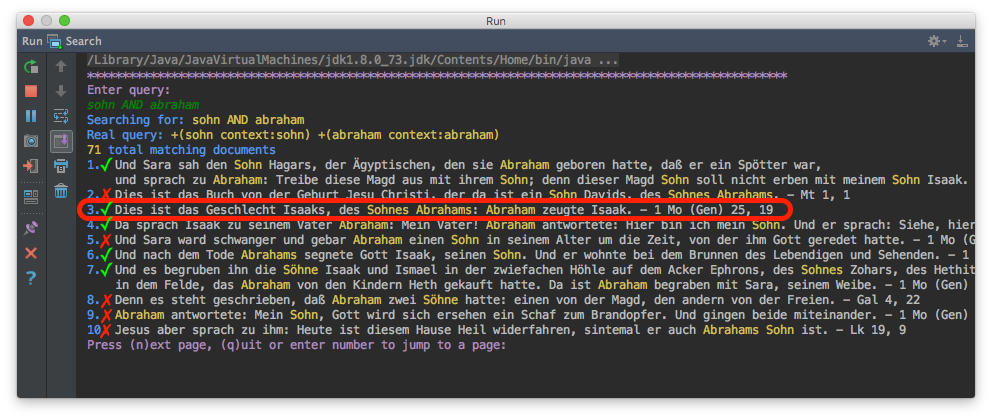
\includegraphics[width=1.0\textwidth]{images/4-comparison/search_result_abraham.png}
	\caption{Resultate der Suche nach dem Namen von Abrahams Sohn}
\end{figure}

Da hier relativ viele Ergebnisse gefunden werden (71 \glspl{glos:documentLabel}), wird hier eine aus dem Web bekannte Variation der Precision und Recall verwendet; die \textit{Precision at K}. Dabei werden nur die ersten K Einträge bewertet. Dies wird oft bei Suchmaschinen angewendet, da der Nutzer meist nur an den ersten Einträgen interessiert ist.
Für die vorliegenden Suchen wird $k = 10$ gesetzt.

\begin{table}[H]
	\centering
	\small\renewcommand{\arraystretch}{1.4}
	\rowcolors{1}{tablerowcolor}{tablebodycolor}
	\captionabove{Suche nach dem Namen von Abrahams Sohn: Precision und Recall}
	%\label{tab:index_abendmahl}
	\begin{tabularx}{0.9\textwidth}{ L{0.22\linewidth} | L{0.1\linewidth} | X }%
		\hline
		& Anzahl & Erklärung \\ \hline \hline
		Relevant: & 1 & Es wird eine Information gesucht, die mehrmals bestätigt werden kann.\\
		Relevant \& gefunden: & 5 & \\
		Fehler: & 5 & \\
		Total Ergebnisse: & 10 & \\
		\hline
		\textbf{Recall:} & \textbf{5} & $= \frac{5}{1} \rightarrow$ 100\% der Resultate wurde gefunden\\
		\textbf{Precision:} & \textbf{0.5} & $= \frac{5}{10}$ \\
		\hline\hline
	\end{tabularx}
\end{table}

Diese Suche ist schwierig zu bewerten, da nur eine Information gesucht ist. Trotzdem können mit diesen Werten verschiedene Suchmaschinen miteinander verglichen werden.

% **********************************************************************************

\newpage
\subsection{Suche nach dem Vers Joh 3,16}
\begin{table}[H]
	\centering
	\small\renewcommand{\arraystretch}{1.4}
	\rowcolors{1}{tablerowcolor}{tablebodycolor}
	%
	\captionabove{Suche: "`Denn so sehr hat Gott die Welt geliebt, ..."'}
	%
	\begin{tabularx}{0.9\textwidth}{ L{0.15\linewidth} | X  }%
		\hline
		Frage: & \textit{Wie heisst der Vers ähnlich: "`Denn so fest hat Gott die Welt geliebt, dass..."'}. Wo steht er?\\
		Anfrage-Typ: & \textit{Vers orientierte Anfrage}\\
		Beschreibung: & Der Nutzer will den genauen Vers inkl. Stellenangabe sehen.\\
		Query: & \textit{denn so fest hat gott die welt geliebt}\\
		Erwartung: & Vers und Stellenangabe:
		"`Also hat Gott die Welt geliebt, daß er seinen eingeborenen Sohn gab, auf daß alle, die an ihn glauben, nicht verloren werden, sondern das ewige Leben haben."' - \textit{Joh 3,16 \gls{lutLabel}}\\
		\hline
	\end{tabularx}
\end{table}

\begin{figure}[H]
	\centering
	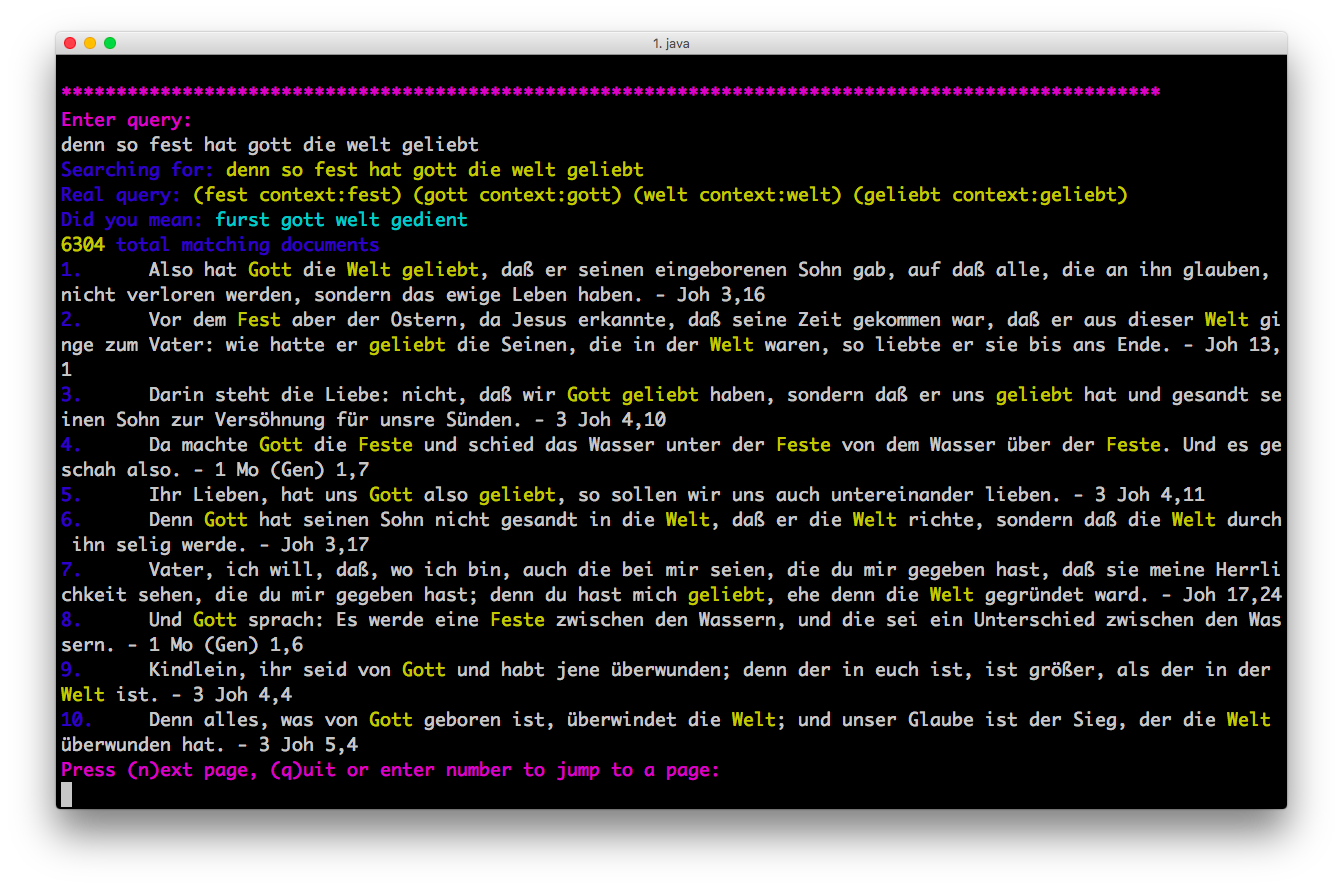
\includegraphics[width=1.0\textwidth]{images/4-comparison/search_result_john3-16.png}
	\caption{Resultate der Suche nach Joh 3,16}
\end{figure}

Für diese Suche macht es wenig Sinn die Precision und den Recall zu berechnen, da es nur genau ein relevantes \gls{glos:documentLabel} gibt, dass gefunden werden kann oder nicht.
Zusätzlich sollte aber die Position des Ergebnisses verglichen werden.
Die Anzahl der Ergebnisse sagt bei dieser Liste mit Ranking nicht viel aus und wird darum ignoriert.

\begin{table}[H]
	\centering
	\small\renewcommand{\arraystretch}{1.4}
	\rowcolors{1}{tablerowcolor}{tablebodycolor}
	\captionabove{Suche nach dem bekannten Vers Joh 3,16}
	%\label{tab:index_abendmahl}
	\begin{tabularx}{0.6\textwidth}{ L{0.4\linewidth} | X }%
		\hline
		Vers gefunden & Ja\\
		Position des Resultates & 1\\
		\textit{Total Ergebnisse} & \textit{6304}\\
		\hline
	\end{tabularx}
\end{table}


% **********************************************************************************
% **********************************************************************************
% **********************************************************************************

\newpage
\section{Bewertung und Vergleich der externen Suchmaschinen}
Es sind drei externe Suchmaschinen bekannt: der BibleServer.com\footcite{BibleServer_Die_Bibel_fr_alle_2016-05-30}, der BibleGateway.com\footcite{BibleGateway_2016-05-30} und die Android App \textit{Bible} von Life.Church \footcite{Bible_Android_Apps_on_Google_Play_2016-05-30}.

Während der Nutzung von BibleServer und BibleGateway wurde bekannt, dass beide Suchmaschinen die exakt selben Resultate liefern.
Auf Grund dessen, wird folgend die BibleServer ignoriert. Die gleichen Kennzahlen treffen aber auch auf die BibleServer-Suchmaschine zu.
Nur die Android App unterstützt ein Ranking. Bei den anderen Suchen werden die Resultate gemäss der traditionellen Reihenfolge der Bibel sortiert dargestellt.

Als Grundlage wird weiterhin überall die \gls{lutLabel} Übersetzung verwendet.


% **********************************************************************************

\subsection{Suche zum Thema Abendmahl}
Beide externe Suchmaschinen verknüpfen standardmässig alle Begriffe mit \textit{AND}. Also lautet das entsprechende Query "`\textit{leib brot}"'.

Das Resultat beider Suchmaschinen (BibleGateway und der Android App) ist beinahe identisch. Die Reihenfolge entspricht der Liste der Bibel App, da wie erwähnt der BibleGateway kein Ranking unterstützt.
\begin{itemize}[noitemsep]
	\item 1 Kor 10,17
	\item Mt 26,26
	\item Mk 14,22
	\item 1 Kor 10,16
	\item 1 Kor 11,27
	\item Lk 22,19
	\item \textit{1 Mo 47,19} $ \rightarrow$ \textit{wird nur von BibelGateway angezeigt}
\end{itemize}

Die Resultate lassen sich wie folgt gruppieren:
\begin{table}[H]
	\centering
	\small\renewcommand{\arraystretch}{1.4}
	\rowcolors{1}{tablerowcolor}{tablebodycolor}
	\captionabove{Externe Suche zum Thema Abendmahl: Gruppierung der relevanten Dokumenten}
	%\label{tab:grouped_results_abendmahl}
	\begin{tabularx}{0.9\textwidth}{ L{0.15\linewidth} | L{0.08\linewidth} | X }%
		\hline
		Bereich & Treffer & Bibelstelle \\ \hline \hline
		Mt 26, 17-29 & 1 & Mt 26,26 \\
		Mk 14, 12-26 & 1 & Mk 14,22\\
		Lk 22, 14-20 & 1 & Lk 22,19\\
		Joh 13, 2-4 & 0 & -\\
		1 Kor 11, 23-27 & 1 & 1 Kor 11,27\\
		\hline
		\textit{andere korrekt} & \textit{1} & 1 Kor 10,16 (war nicht explizit verlangt)\\
		\textit{andere falsch} & \textit{1 | (2)} & 1 Kor 10,17; (1 Mo 47,19 nur beim BibleGateway)\\
		\hline\hline
		\textbf{Total} & \textbf{6 | (7)} & Wert in Klammern gilt für den BibleGateway\\
		\hline
	\end{tabularx}
\end{table}

Daraus folgt für die Precision und den Recall die Werte in \cref{tab:index_abendmahl_foreign}
\begin{table}[H]
	\centering
	\small\renewcommand{\arraystretch}{1.4}
	\rowcolors{1}{tablerowcolor}{tablebodycolor}
	\captionabove{Externe Suche zum Thema Abendmahl: Precision und Recall}
	\label{tab:index_abendmahl_foreign}
	\begin{tabularx}{0.9\textwidth}{ L{0.22\linewidth} | L{0.2\linewidth} | X }%
		\hline
		& Anzahl & Erklärung \\ \hline \hline
		Relevant: & 5 & \\
		Relevant \& gefunden: & 6 & 1+1+1+0+3\\
		Relevant \& gefunden (gruppiert): & 4 & Gruppen à: 1, 1, 1, 0, 3 Dokumente\\
		Fehler: & 1 & \\
		Total Ergebnisse: & 7 & \\
		\hline
		\textbf{Recall:} & \textbf{0.8} & $= \frac{4}{5}$\\
		\textbf{Precision:} & \textbf{0.83 | (0.71)} & $=\frac{5}{6}$ für die Android App und $=\frac{5}{7} $ für den BibleGateway\\
		\hline\hline
	\end{tabularx}
\end{table}

\subsubsection{Vergleich der Suchmaschinen}
Verglichen mit der umgesetzten Suche, fallen folgende Unterschiede auf:
\begin{itemize}[noitemsep]
	\item Es werden lediglich Verse gefunden, die alle Suchbegriffe beinhalten.
	\item Die Precision bei beiden externen Suchmaschinen ist deutlich besser, als bei der umgesetzten Suche.
		Dies ist so, weil die umgesetzte Suche auch Verse anzeigt, die nicht vollständig zutreffen. Doch durch das unterstütze Ranking kann das Ergebniss trotzdem sinnvoll gelesen werden.
	\item Das \gls{glos:documentLabel} ist auf einen Vers beschränkt. Sätze die sich über mehrere Verse erstrecken und beide Suchbegriffe beinhalten werden nichts gefunden (z.B. 1 Kor 11,23-24).
	Gemäss der Definition des Queries, sollte jene Stellen ebenfalls zu den relevanten Dokumenten gehören.
	\item Der weitere Kontext der Nachbarsversen wird bei beiden externen Suchmaschinen ebenfalls ignoriert, was bei der umgesetzten Suchmaschine den Vorteil bringt, dass dies beim Ranking berücksichtigt wird.
	Zudem erscheinen jene Verse die nur im Nachbar die Begriffe beinhalten, trotzdem am Ende der Resultat Liste, gleichzeitig werden so mehrere Ergebnisse gefunden, durch die die Precision verschlechtert wird.
\end{itemize}

% **********************************************************************************

\subsection{Suche nach dem Namen von Abrahams Sohn}
Das Resultat umfasst 28 \glspl{glos:documentLabel} in der abgebildeten Reihenfolge der Android App.
Die Top 10 werden hier aufgelistet.
\begin{table}[H]
	\centering
	\small\renewcommand{\arraystretch}{1.4}
	\rowcolors{1}{tablerowcolor}{tablebodycolor}
	\captionabove{Externe Suche nach dem Namen von Abrahams Sohn: Auswertung der Ergebnisse}
	%\label{tab:index_abendmahl_foreign}
	\begin{tabularx}{0.9\textwidth}{ R{0.1\linewidth} | L{0.2\linewidth} | X }%
		\hline
		Rang & Vers & Treffer \\ \hline \hline
		1. & 1. Mo 21,2 & falsch\\
		2. & 1. Mo 17,23 & (wahr, aber nicht der gesuchte Sohn)\\
		3. & 1. Mo 25,19 & wahr\\
		4. & 1. Mo 21,11 & falsch\\
		5. & Mt 1,1 & falsch\\
		6. & 1. Mo 21,10 & wahr\\
		7. & Lk 3,34 & wahr\\
		8. & 1. Mo 17,26 & (wahr, aber nicht der gesuchte Sohn)\\
		9. & 1. Mo 21,3 & wahr\\
		10. & 1. Mo 21,5 & wahr\\
		\hline
	\end{tabularx}
\end{table}


\begin{table}[H]
	\centering
	\small\renewcommand{\arraystretch}{1.4}
	\rowcolors{1}{tablerowcolor}{tablebodycolor}
	\captionabove{Externe Suche nach dem Namen von Abrahams Sohn: Precision und Recall}
	%\label{tab:index_abendmahl}
	\begin{tabularx}{0.9\textwidth}{ L{0.22\linewidth} | L{0.1\linewidth} | X }%
		\hline
		& Anzahl & Erklärung \\ \hline \hline
		Relevant: & 1 & Es wird eine Information gesucht, die mehrmals bestätigt werden kann.\\
		Relevant \& gefunden: & 7 & \\
		Fehler: & 3 & \\
		Total Ergebnisse: & 10 & \\
		\hline
		\textbf{Recall:} & \textbf{7} & $= \frac{7}{1} \rightarrow$ 100\% der Resultate wurde gefunden\\
		\textbf{Precision:} & \textbf{0.7} & $= \frac{7}{10}$ \\
		\hline\hline
	\end{tabularx}
\end{table}

\subsubsection{Vergleich der Suchmaschinen}
Verglichen mit der umgesetzten Suchmaschine, fallen folgende Unterschiede auf:
\begin{itemize}[noitemsep]
	\item Die Precision bei der externen Suchmaschine ist höher, als bei der umgesetzten Suchmaschine. \todo{wieso?}
	\item Auch bei dieser externen Suchmaschine können nur Verse und nicht ganze Sätze gefunden werden.
	\item Der weitere Kontext der Nachbarsversen wird ebenfalls ignoriert.
	Dies sollte aber nicht der Grund sein, warum die umgesetzte Suchmaschine eine tiefere Precision hat. (In der Resultatmenge hat es nur zwei Verse die Nachbarsversen sind, beide beinhalten alle Suchwörter).
\end{itemize}


% **********************************************************************************

\subsection{Suche nach dem Vers Joh 3,16}
Bei der Query "`denn so fest hat gott die welt geliebt"' finden beide externe Suchmaschinen (der BibleGateway und die Android App) keine Ergebnisse.
Der BibleGateway unterstützt eine Suche nach "`ANY word"', was aber sehr viele Resultate zur Folge hat (16'890 Resultate), durch das fehlende Ranking ist das Ergebnis wertlos.

\subsubsection{Vergleich der Suchmaschinen}
Verglichen mit der umgesetzten Suchmaschinen, fallen folgende Kriterien auf:
\begin{itemize}[noitemsep]
	\item BibleGateway unterstützt anscheinend kein \textit{Stop Words Filtering}.
	\item Ein Ranking ist ein notwendiges Features, wenn es viele zutreffende Dokumente gibt. Ansonsten ist die Suchmaschine in diesen Fällen vollkommen wertlos.
\end{itemize}

